\chapter{Introduction}
This chapter gives a short introduction about project motivations,
cryptographic protocols, and proof assistant. 
\section{Objectives and Project Motivations}
Cryptographic protocols are intended to let principals communicate
securely over a communication protocol which are designed to provide
various kinds of security assurances. An important security goal of
cryptographic protocol is authentication, the act of confirming the
truth of an attribute of a datum or entity like verifying freshness of
a nonce. Many research papers about authentication have published. One
of them is “Authentication Tests and the Structure of Bundles” by
Joshua Guttman and Javier Thayer. The main idea of authentication
tests is that if a principal in a cryptographic protocol creates and
transmits a message containing a new value $v$, and later receives $v$
back in a different cryptographic context then it can be concluded
that some principal processing the relevant key has received and
transformed the message in which  was emitted. The authentication
tests themselves are easy to apply but the proof justifying them are
more complicated \cite{Guttman}. Though authentication tests are proved in the paper, they have not been formally verified.  As we know that once lemma or a
theorem has been proved in some proof assistant language like Coq, we
will have a very strong assurance that it is true - much more than
what we usually have when doing a pen-and-paper proof. In addition, we found that there are few papers and projects using Coq to verify security goal of cryptographic protocols and to particularly formalize strand spaces, which is a well-known approach to cryptographic protocols.

In this project we will prove authentication tests under strand space formalism approach by using the Coq proof assistant. First, we will formalize strand spaces and all stuffs needed for proving authentications tests like components,transformation paths, penetrable keys. Then, we will give detailed formal proofs of all relevant lemmas, theorems, and finally authentication tests.

This project will help researchers in security area have more
confidence in using the result of authentication tests since they are
formally verified. Our implementation is modular so that researchers
can easily extract certain modules for their purpose. For example, the
formalization of strand spaces can be used as a frame work for later
research using strand space approach.

\section {Reasoning about Cryptographic Protocols}
Cryptographic protocols are programs that aim at securing communications on insecure networks, such as Internet, by relying on cryptographic primitives. Even when cryptographic protocols have developed carefully by experts and also reviewed thoughtfully by other experts, the design of cryptographic protocols may contain some bugs possibly causing them unusable \cite{thayer1998strand}. For instance, in the Needham-Schroeder public-key protocol, a flaw (using man in the middle attack method) was found by Lowe 17 years after its publication. Although much progress has been made, current cryptographic protocols still contains a lot of flaws, which can cause serious consequences. Moreover, security errors cannot be detected by functional software testing because they appear only in the presence of a malicious adversary. Automatic tools can therefore be very helpful in detecting and also verifying the correctness of security protocols.  A lot of tools for verifying and analyzing cryptographic protocols have been developed like ProVerfi, SATMC, PVS, and CPSA. Hence, security protocol verification has been a very active research area since 1990s.

There are several techniques for proving protocol correctness. Two common approaches in this area are symbolic and computational models. Symbolic model approach relies on specifications while computational model approach relies on implementations. Another well-known approach is strand space model, developed by Joshua D. Guttman, Javier Thayer F´abrega, and Jonathan C. Herzog. This approach has several advantages as followings. 
\begin{itemize}
\item It gives a clear semantics to the assumption that certain data
items, such as nonces and session keys, are fresh, and never arise in more
than one protocol run \cite{ss}.
\item It provides an explicit model of the possible behaviors of a system
penetrator; this allows to develop general theorems that bound the
abilities of the penetrator, independent of the protocol under study \cite{ss}.
\item It allows various notions of correctness, involving both secrecy
and authentication, to be stated and proved \cite{ss}.
\item The approach leads to detailed insight into the reasons why
the protocol is correct, and the assumptions required. Proofs are simple
and informative: they are easily developed by hand, and they help to
identify more exact conditions under which we can rely on the protocol
\cite{ss}.
\end{itemize} 
We will describe in details strand spaces in the next chapter. %citation %
 
\section {Proof Assistants}
Proof assistants (interactive theorem provers) are computer systems that allow a user to do mathematics on a computer, but not so much the computing (numerical or symbolical) aspect of mathematics but the aspects of proving and defining. So a user can set up a mathematical theory, define properties and do logical reasoning with them. In many proof assistants one can also define functions and compute with them, but their main focus is on doing proofs. As opposed to proof assistants, there are also automated theorem provers. These are systems consisting of a set of well chosen decision procedures that allow formulas of a specific restricted format to be proved automatically. Automated theorem provers are powerful, but have limited expressivity, so there is no way to set-up a generic mathematical theory in such a system.

There are a lot of proof assistant systems like Isabelle, Coq, PVS, NuPRL. Out of them, Coq seems to be the most powerful system that supports a lot of features: higher-order logic, dependent types, proof automation, proof by reflection, code generation, and having a small kernel. The Coq proof assistant is distinguished from the other. That is one main reason that I and my advisor chose to use Coq instead of another proof assistant.
%\begin{table}
%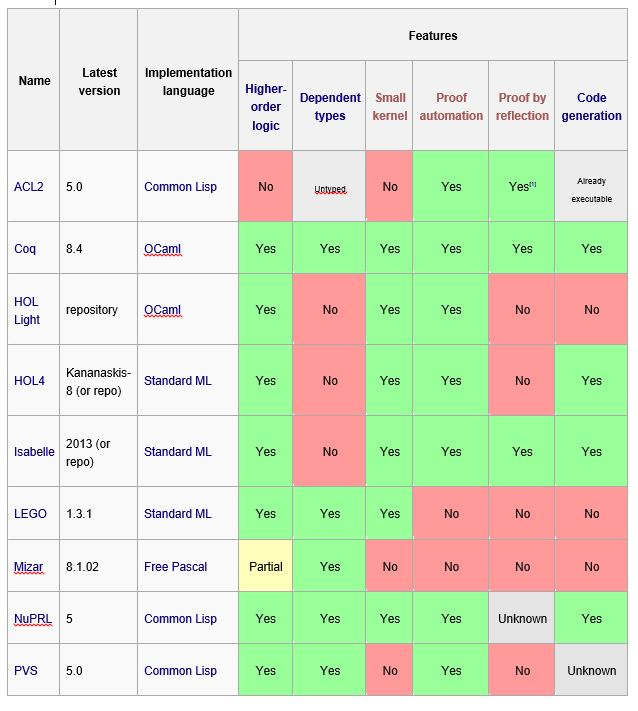
\includegraphics[scale=0.8]{ProofAssistant.jpg}
%\caption{Comparison of proof assistant systems}
%\end{table}

In addition, proving using Coq provides numerous advantages over paper-and-pencil proofs. First, Coq can mechanically check our proofs, hence it provides much greater confidence on our formalization and on the correctness of our theorems. Second, because all proofs in Coq are constructive, we can automatically extract certified implementations of all our theories. This provides runnable tools (for free!) and give us confidence in the tools as well. Finally, a mechanized representation is more valuable to others who can much more easily
adapt our work to related projects and obtain high confidence in the results.


\chapter{Background}

\section{Strand Space Overview}
In this section, we briefly summarize the ideas behind the strand space model. The Coq development in the next chapter will provide precise definitions.

A strand spaces is a set of strands; one may think of a strand space as containing all legitimate executions together with all the actions that a penetrator may apply to the messages contained in these executions.

A strand is a sequence of events that a single principal, either a legitimate principal or a penetrator, may engage in. The height of a strand is the number of nodes on that strand. Each strand is a sequence of message transmissions and receptions with specific values such as nonces and keys. Transmission of a term $t$ is represented as $+t$ and reception of a term $t$ is represented as $-t$. Each element of a strand is called a node. Given a strand $s$, $(s,i)$ is the $i^th$ node on $s$. We say that $n \Rightarrow n'$ if $n=(s,i)$ and $n'=(s,i+1)$. Thus, the relation $\Rightarrow^+$ between two nodes is the transitive closure of the relation $\Rightarrow$. The relation $n \rightarrow n'$ represents the inter-strand communication; it means that $term(n)=+t$ and $term(n')=-t$; here $term(n)$ denotes the signed (unsigned) message at the node $n$.

Let $A$ be the set of all possible messages that can be exchanged between principals in a protocol. We call elements of $A$ terms. $A$ is freely generated from two disjoint sets, set of texts $T$ and set of cryptographic keys $K$, by concatenations $encr : K \times A \rightarrow A$ and encryptions $join : A \times A \rightarrow A$. Hence, $A$ is closed under concatenation and encryption. The set $K$ is equipped with an injective unary operator $inv : K \rightarrow K$ which maps each member of asymmetric key pair to the other and maps a symmetric key to itself.

A signed term is a pair of a sign $\sigma \in {+,-}$ and a term t, written either $<\sigma,t>$ or $+t$ or $-t$.

A term $t_1$ is a subterm of another term $t_2$, denoted as $t_1 \sqsubset t_2$, if we can get $t_2$ from $t_1$ by repeatedly concatenating with arbitrary terms and encrypting with arbitrary keys. For example, $A, N_a$ are subterms of ${|N_aA|}_K$ but $K$ is not.

Another important concept under strand space is origination. We say that a term t originates at a node n if n is a transmission node, $t \sqsubset term(n)$, and t is not a sub-term of any earlier node of $n$; hence, $n$ is the first node in its strand includes $t$. A node is called uniquely originating if it is originated on only one node over all strands.

A bundle is a casually well-founded collection of nodes and two relations $\Rightarrow$ and $\rightarrow$. It represents the actual protocol interactions. In a bundle, when a a strand receives a message $m$, there is a unique node transmitting $m$ from which the message was immediately  received. In contrast, when a strand transmits a message $m$, many strands or none may immediately receive $m$. The height of a strand in a bundle is the number of nodes on the strand that are in the bundle.

The penetrator's powers are characterized by the set of compromised keys which are initially known to penetrator, and a set of penetrator strands that allow the penetrator to generate new messages. The set of compromised keys typically would contain all public keys, all private keys of penetrators, and all symmetric keys initially shared between the penetrator and principals playing by the protocol rules. The atomic actions available to penetrator are encoded in a set of penetrator strands. We partition penetrator strands according to the operations they exemplify. E-strands encrypt when given a key and a plain-text; D-strands decrypt when given a decryption key and matching cipher-text; C-strands concatenate terms; S-strands separate terms; M-strands emit known atomic text or guess; and K-strands emit keys from a set of known keys.

Important units for protocol correctness are components. A term $t$ is a component of another term $t'$ if $t \sqsubset t'$, t is nt a concatenated term, and for every $s \neq t$ such that $t \sqsubset s \sqsubset t'$, $s$ is a concatenated term. Thus, a component is either atomic value or an encryption. A term $t$ is new at a node $n=<s,i>$ if t is a component of $term(n)$ but $t$ is not a component of node $<s,j>$ for every $j < i$. A component is new even if it has occurred earlier as a nested subterm of some larger component. When a component occurs new in a regular node but was a subterm of some previous node, then the principal executing that strand has done some cryptographic work to extract it as a new component\cite{Guttman}. 

\section{The Coq Proof Assistant Overview}
\subsection{What is Coq?}
We briefly describe what the Coq proof assistant is in this section.

The Coq system is a computer tool for mechanically verifying theorem
proofs, and at the same time a functional programming language with a
powerful type system.

Once you have proved something in Coq, you
have strong assurance that it is true - more than what you usually
have when doing a pen-and-paper proof. These theorems may concern
usual mathematics, proof theory, or program verification. The Coq
proof assistant is very powerful and expressive both for reasoning
and programming. We can construct from simple terms and write simple
proofs to building whole theories and complex algorithms. It provides
an environment for defining objects (integers, sets, trees,
functions...), making statements using logical connectives and basic
predicates, and writing proofs. It also provides program extraction
towards Haskell and Ocaml for efficient execution of algorithms and
linking with other libraries.

The Coq compiler automatically checks the correctness of definitions
(well-formed sets, terminating functions...) and of proofs \cite{paulin2012introduction}.

As a proof assistant, Coq is similar to higher order logic (HOL)
systems, a family of interactive theorem prover based on Church's HOL
including Isabelle, PVS... Unlike these systems, Coq is based on
intuitionistic type theory. Consequently, it is closer to Epigram, and
NuPrl... The common properties of these system are that functions are
programs that can be computed and not just binary relation.  Coq can
be used from standard teletype-like shell window but preferably
through the graphical user interface called CoqIde. Coq is not an
automated theorem prover which means that it does not automatically
prove theorems. However, it can be considered as a semi-automated
theorem prover since it includes many automatic theorem proving tatics
and various decision procedures. It greatly simplifies the development
of formal proofs by automating some aspects of it.

Under programming language point of view, Coq implements dependently
typed functional programming language, while under logical system, it
implements a higher-order type theory \cite{bertot2004coq}. Coq exploits the notion of Curry-Howard isomorphism - the correspondence between proofs and
programs. The relation between a proof and the statement it proves is
the same as the relation between a program and its type. At the level
of proofs and programs, we have the following correspondence
summarized in Table 1.1.
\begin{table}[h!]
\begin{center}
	\begin{tabular}{|c|c|}
		\hline
		Logic side & Programming side \\ \hline  \hline
		hypothesis & free variables \\ \hline
		implication elimination & application \\ \hline
		implication introduction & abstraction \\ \hline
	\end{tabular}
\end{center}
\caption{}
\end{table}

And Table 1.2 summaries the correspondence at the level of terms and types.
\begin{table}[h!]
\begin{center}
	\begin{tabular}{|c|c|}
		\hline
			Logic side & Programming side \\ \hline 
			universal quantification & generalised function space \\ \hline
			existential quantification & generalised cartesian product \\ \hline
			implication	& function type \\ \hline
			conjunction	& product type \\ \hline
			disjunction	& sum type \\ \hline
			true formula & unit type \\ \hline
			false formula & bottom (empty) type \\ \hline
	\end{tabular}
\end{center}
\caption{}
\end{table}
The correspondence says that, for example, implication behaves the same as a
function type, conjunction as product type, and disjunction as sum
type. %
The assertion $T:\tau$ means that the term $T$ is of type $\tau$ or
equivalently that $T$ is a proof of the proposition $\tau$.   A type $A \rightarrow B$
is the type of a function that associates  a term of type $B$ to any
term of type $A$, while a proof of $A \rightarrow B$ is a term of that
type or a term of the form $\lambda x.t$ where x is a proof of $A$ and
t is a proof of $B$. 

There is usually a syntactic distinction between types and terms in
most type theories. However, types and terms are defined as the same
syntatic structure so everything even type is a term in
Coq. Consequently, all objects have a type:  atomic types, types for
functions, types for proofs, types for types. When manipulated as
terms, types are themselves a type which is a constant of the language
called a sort. Prop and Set are the two base sorts. The sort Prop is
the universe of propositions. The sort Set intends to be the type of
small sets and includes data types such as booleans, natural numbers,
and but also includes products, subsets, function type over these data
types.

The original Coq system was based on the Calculus of Constructions
(CoC). %
Version 7 was based on a generalization of CoC, the Calculus of Inductive
Constructions (CIC). %
Since version V8 it is based on a weaker calculus, namely Predicate
Calculus of Inductive Constructions (pCIC). %
[citation] 
The language of CIC also has typed terms, conversion rules,
derived rules, and (co)inductive definitions.

\subsection{Coq Architecture}
Coq have two levels architecture - kernel and environment. A relatively small kernel based on a language with few primitive constructions (sorts, functions, inductive definitions, product types...) and a limited number of rules for type checking and computation. On top of the kernel, there is a rich environment to help designing theories and proofs. This environment offers mechanism like user extensible notations, tatics for proof automation, libraries... Any definition or proof defined in the environment is ultimately checked by the kernel so the environment can be used and extended safely \cite{paulin2012introduction}.

As a Coq user, using high level constructions will help to solve a problem quickly. However, it might also important to understand the underlying low level language in order to develop new functionalities and to better control how certain constructions work. 
 
%\chapter{Strand Space Formalization}%
\input{Message_Algebra}
\input{Strand_Spaces}
\input{Strand_Library}
\input{Authentication_Tests_Library}
\input{Authentication_Tests}
%\chapter{Authentication Tests}%

\chapter{Conclusion and Future Work}

%%% Local Variables:
%%% mode: latex
%%% TeX-master: "Report"
%%% End:
